\documentclass[border=10pt]{standalone}
\usepackage{tikz}
\usetikzlibrary{arrows.meta, decorations.pathmorphing}

\begin{document}
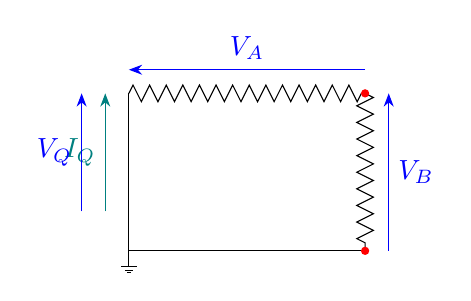
\begin{tikzpicture}[> = Stealth]

% Voltage source vertical line
\draw (0,0) -- (0,2);

% Resistors with zigzag decoration
\draw[decorate, decoration={zigzag, amplitude=3pt, segment length=6pt}] (0,2) -- (3,2);
\draw[decorate, decoration={zigzag, amplitude=3pt, segment length=6pt}] (3,2) -- (3,0);

% Ground connection
\draw (3,0) -- (0,0);

% Ground symbol
\draw (0,0) -- (0,-0.2);
\draw (-0.1,-0.2) -- (0.1,-0.2);
\draw (-0.05,-0.25) -- (0.05,-0.25);
\draw (-0.025,-0.275) -- (0.025,-0.275);

% Connection dots
\fill[red] (3,2) circle (1.5pt);
\fill[red] (3,0) circle (1.5pt);

% Voltage and current arrows
\draw[blue, ->] (3, 2.3) -- (0, 2.3) node[midway, above] {$V_A$};
\draw[blue, ->] (3.3, 0) -- (3.3, 2) node[midway, right] {$V_B$};
\draw[teal, ->] (-0.3, 0.5) -- (-0.3, 2) node[midway, left] {$I_Q$};
\draw[blue, ->] (-0.6, 0.5) -- (-0.6, 2) node[midway, left] {$V_Q$};

\end{tikzpicture}
\end{document}